\chapter{ESP8266 Minimum System}

\section{Tujuan}
\begin{enumerate}
    \item Mempraktikkan teknik penyolderan SMD untuk membangun Minimum System pada mikrokontroler ESP8266.
    \item Memahami karakteristik dan kebutuhan khusus dalam penyolderan komponen SMD.
    \item Mendapatkan keahlian dalam menangani alat solder untuk komponen elektronik ukuran kecil.
    \item Mengembangkan kemampuan untuk membaca skematik dan menerapkannya pada pembuatan prototipe elektronik.
    \item Memahami mekanisme cara menanamkan program ke ESP8266.
\end{enumerate}

\section{Dasar Teori}
Minimum System ESP8266 merupakan papan pengembangan yang dirancang untuk memudahkan penggunaan mikrokontroler ESP8266. ESP8266 sendiri adalah mikrokontroler dengan kemampuan Wi-Fi dan Bluetooth terintegrasi yang sering digunakan untuk proyek IoT (Internet of Things). Dalam penyolderan ESP8266, komponen elektronik dipasang langsung ke permukaan PCB tanpa menggunakan kaki atau pin melalui lubang. 

Penyolderan SMD memerlukan presisi dan kecermatan karena ukuran komponen yang sangat kecil dan pad yang berdekatan satu sama lain. Penggunaan stencil dalam proses penyolderan SMD memungkinkan aplikasi pasta solder yang seragam dan akurat, yang sangat penting untuk mencegah short-circuit pada pad-pad yang berdekatan.

Proses penyolderan SMD untuk ESP8266 melibatkan langkah-langkah seperti penyiapan stencil, aplikasi pasta solder, penempatan komponen dengan pinset atau vacuum pickup tool, dan penyolderan menggunakan solder ujung halus atau hot air rework station. Pemeriksaan visual dan pengujian fungsional dilakukan setelah penyolderan untuk memastikan kualitas sambungan dan fungsi rangkaian secara keseluruhan.

\section{Tugas Pendahuluan}
\begin{enumerate}
    \item Install Visual Studio Code 
    \item Install ekstensi PlatformIO pada Visual Studio Code 
    \item Download firmware dari \url{https://its.id/m/wortel-firmware} lalu build project menggunakan vscode + Platformio sampai success.
\end{enumerate}

\section{Alat dan Komponen}
\subsection{Alat}
\begin{enumerate}
    \item Soldering kit
    \item Timah 0.8 mm
    \item Power source
    \item Sikat 
    \item IPA (Isopropyl alcohol)
    \item Flux
    \item Solder Pasta
    \item Stencil Holder
    \item Stencil
    \item Multimeter
    \item USB to TTL
\end{enumerate}

\subsection{Komponen}
\begin{enumerate}
    \item Minimum System ESP8266 Kit
\end{enumerate}

\section{Eksperimen 1: Stencil dan Aplikasi Pasta Solder}
\begin{enumerate}
    \item Siapkan stencil dan pasta solder.
    \item Posisikan pcb di atas stencil holder.
    \begin{figure}[H]
        \centering
        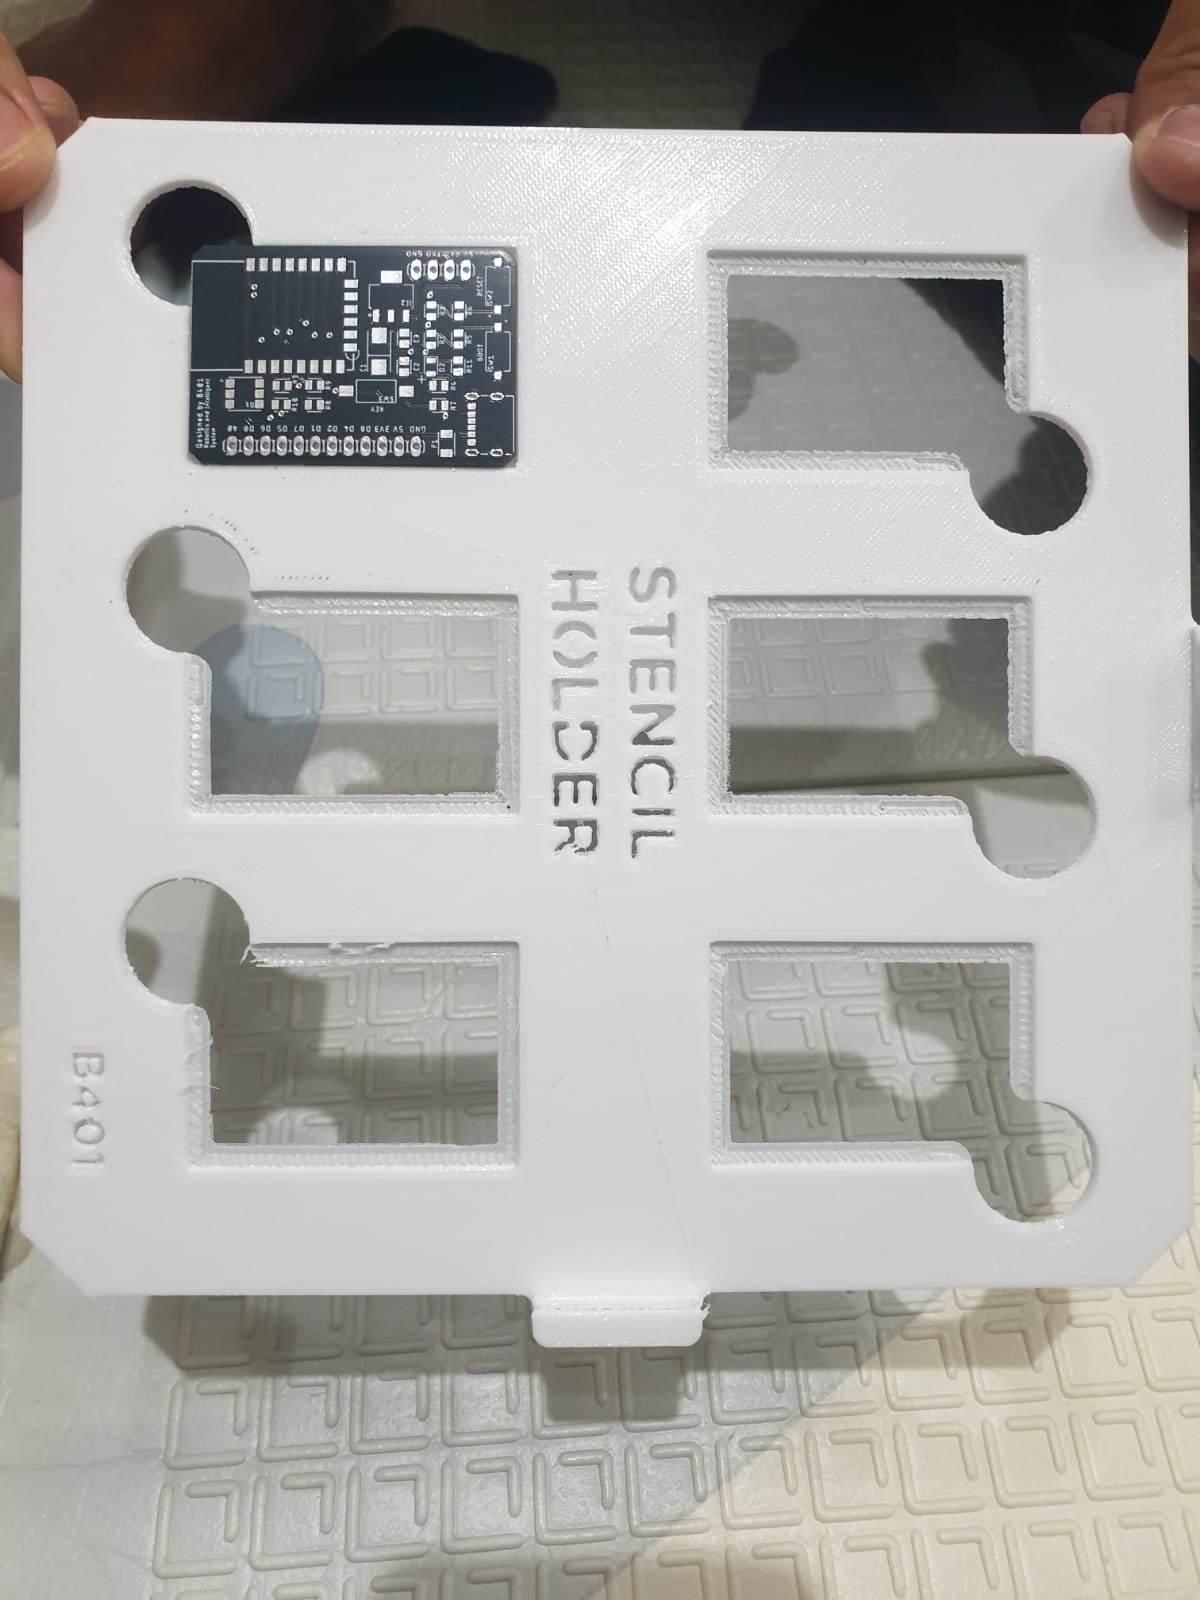
\includegraphics[width=0.4\linewidth]{P4/img/1_board_minsys_ke_holder_stencil.jpeg}
        \caption{Penempatan Board di Stencil}
        \label{fig:PenempatanBoarddiStencil}
    \end{figure}
    \item Letakkan stencil di atas PCB dan pastikan posisi stencil tepat di atas pad.
    \begin{figure}[H]
        \centering
        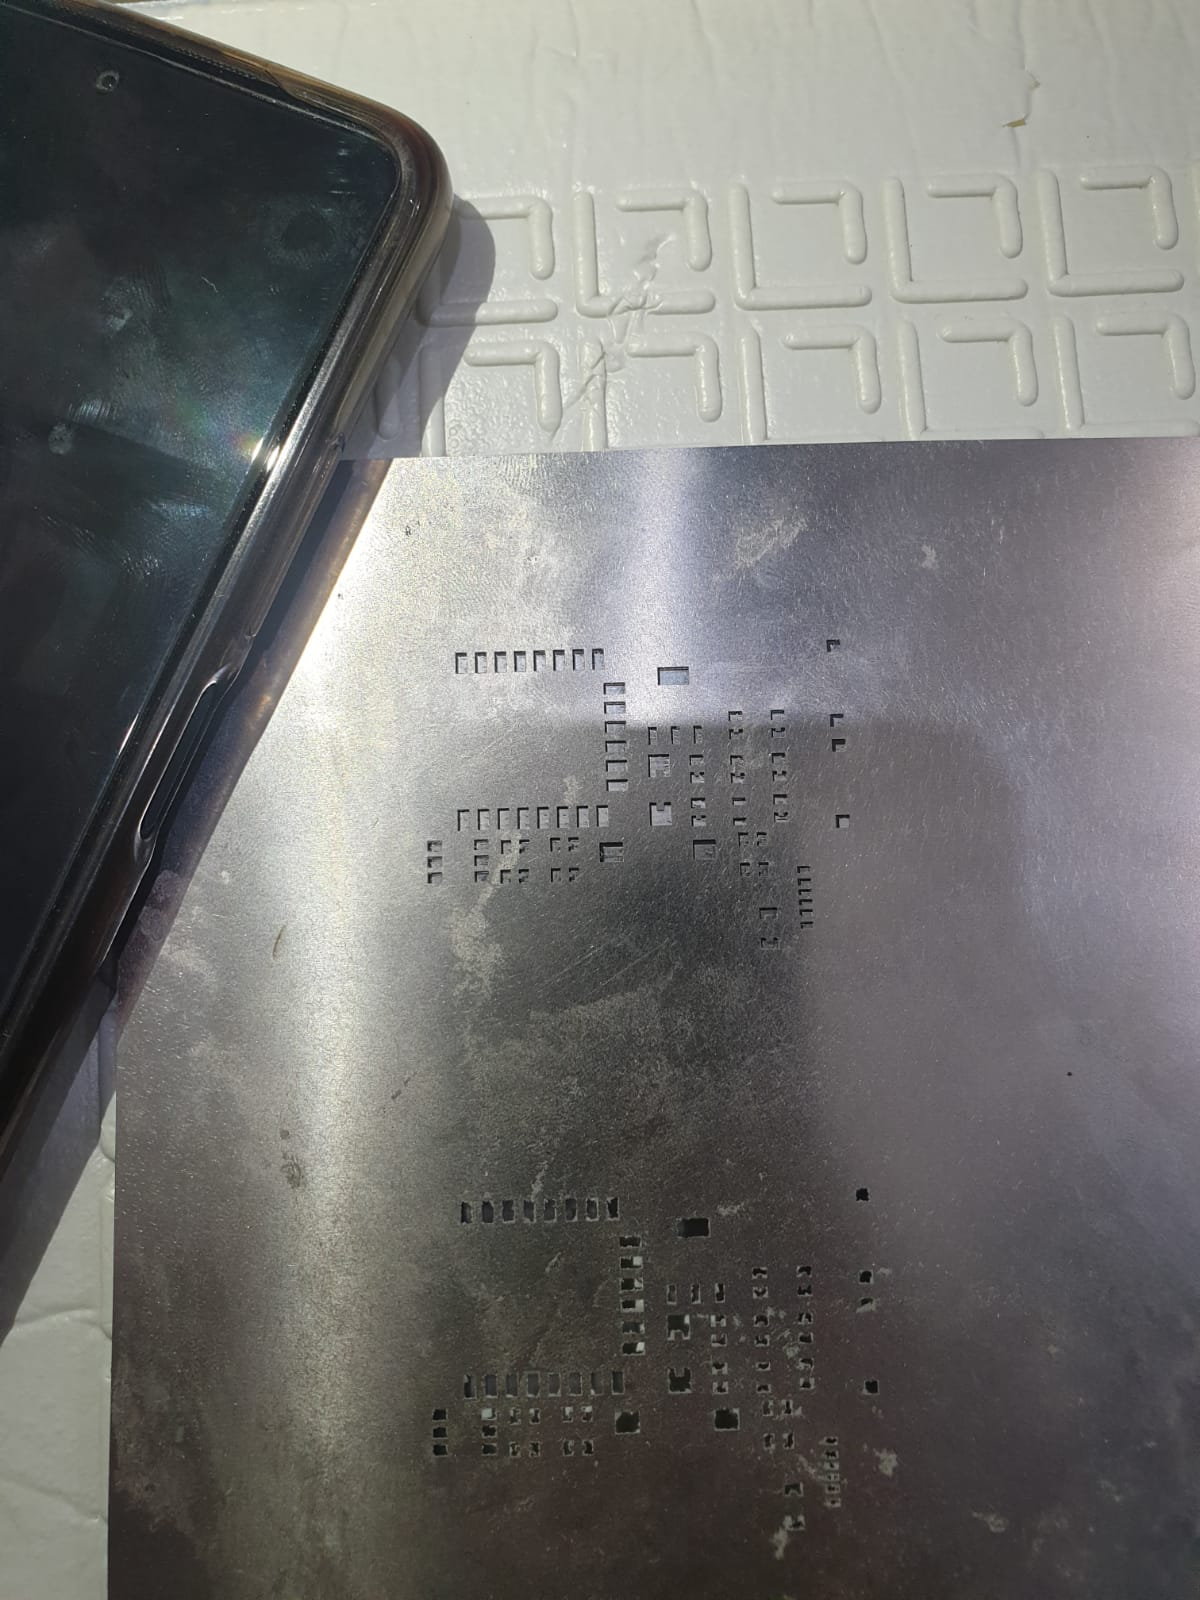
\includegraphics[width=0.4\linewidth]{P4/img/2_pastikan_stencil_pas.jpeg}
        \caption{Stencil Tepat di Atas Pad}
        \label{fig:StencilTepatdiAtasPad}
    \end{figure}
    \item Tuangkan solder pasta ke stencil.
    \begin{figure}[H]
        \centering
        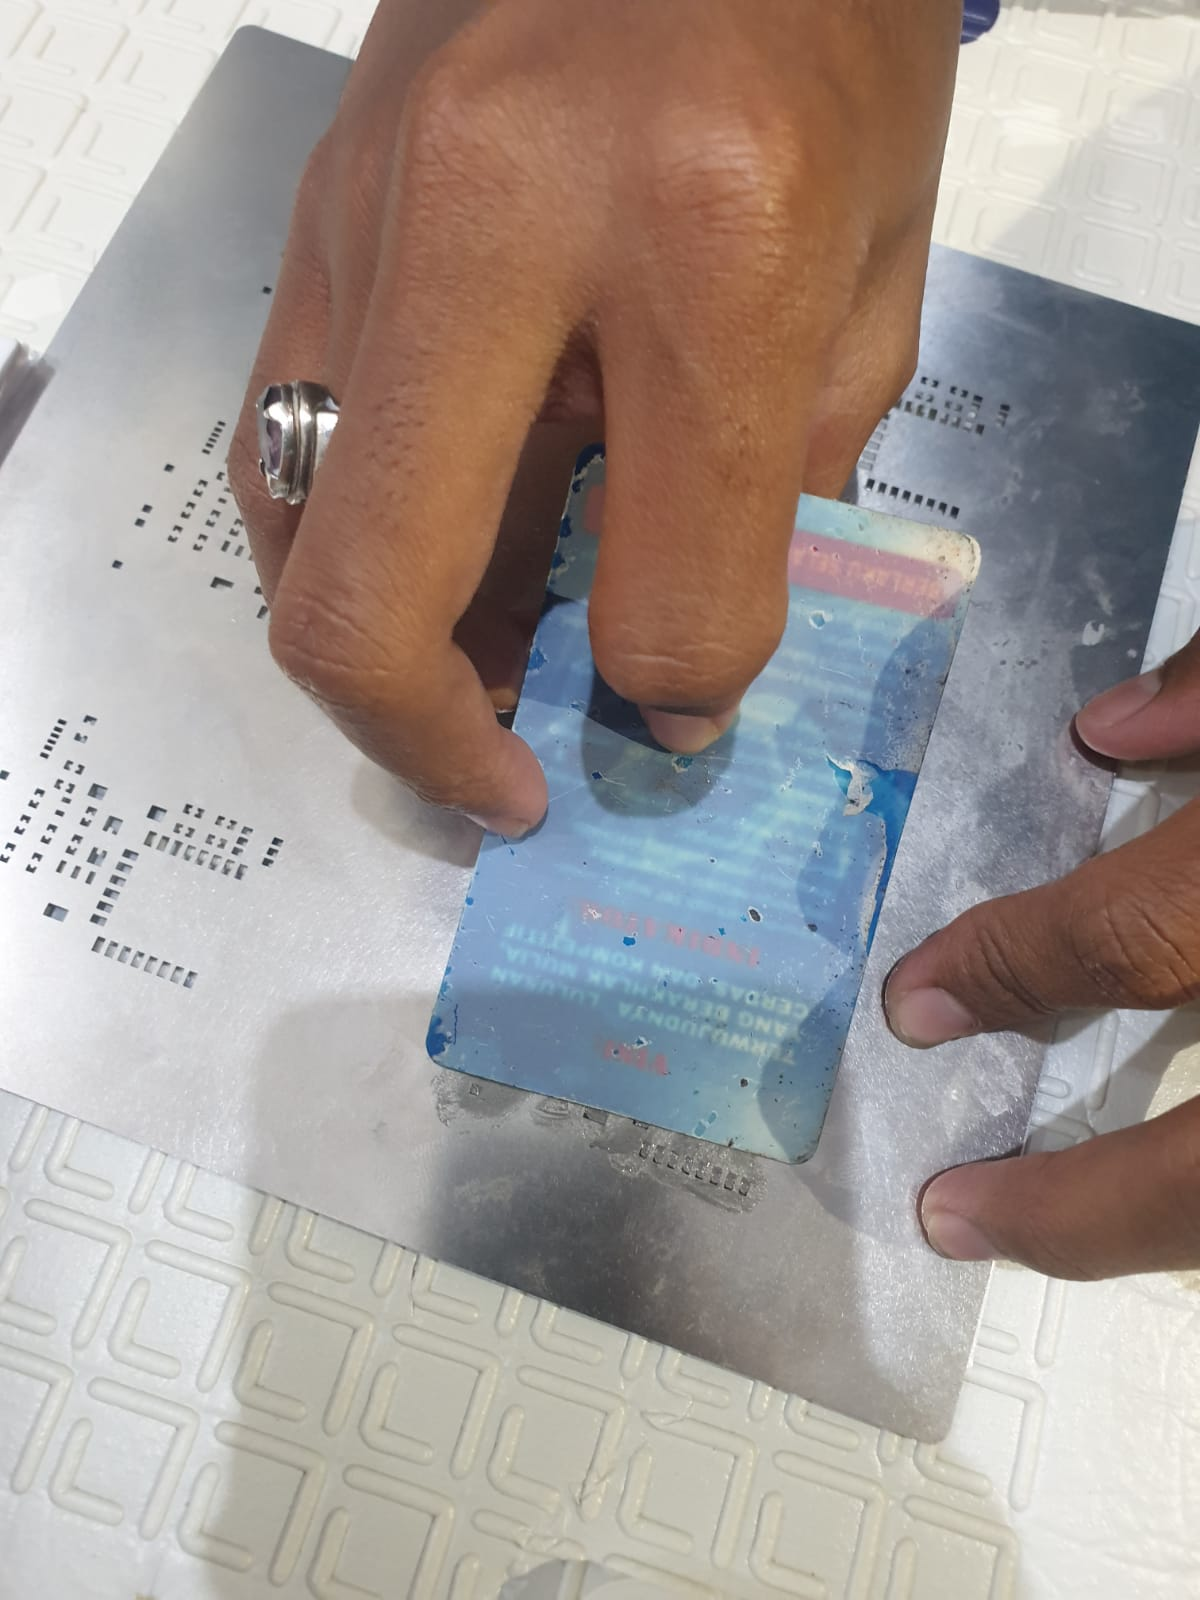
\includegraphics[width=0.4\linewidth]{P4/img/3_taruh_solder_pasta_lalu_ratakan.jpeg}
        \caption{Taruh Pasta Solder}
        \label{fig:TaruhPastaSolder}
    \end{figure}
    \item Ratakan dengan menggunakan spatula.
    \item Bersihkan sisa pasta solder pada stencil.
    \item Periksa hasil aplikasi pasta solder pada PCB.
    \begin{figure}[H]
        \centering
        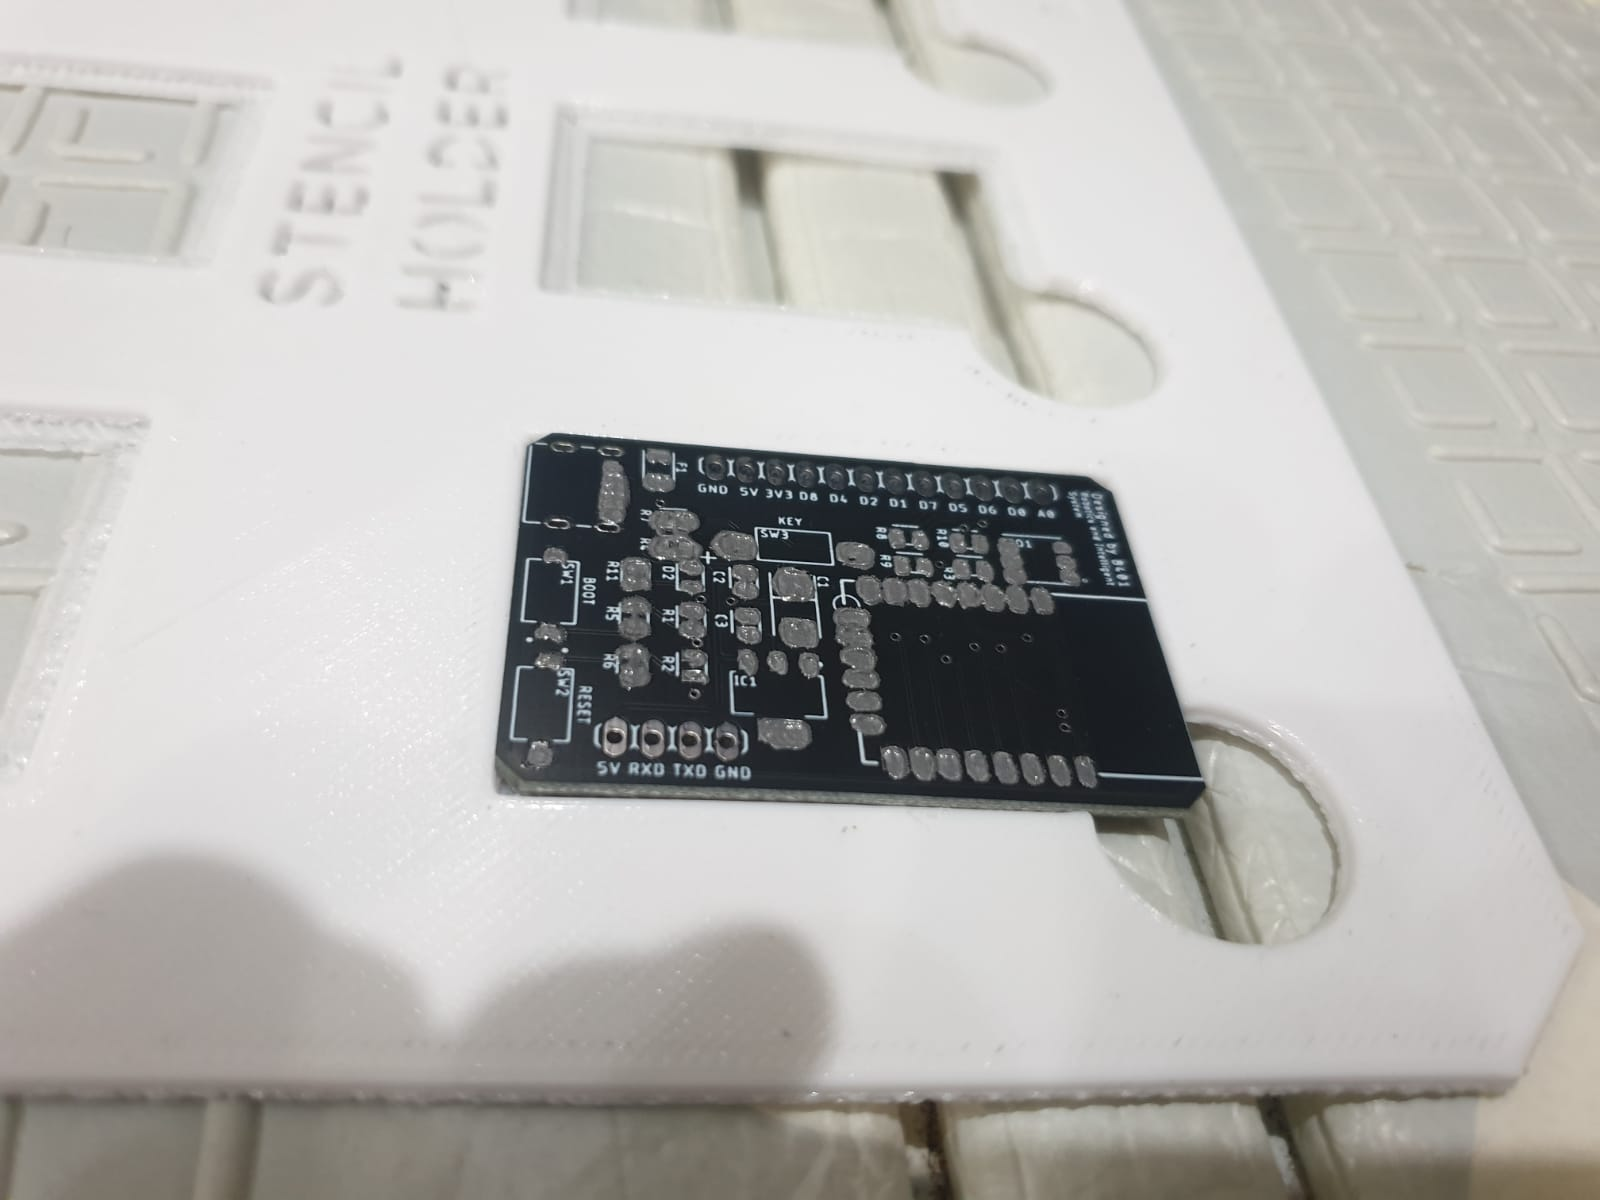
\includegraphics[width=0.4\linewidth]{P4/img/4_keadaan_board_setelah_dipasang_pasta.jpeg}
        \caption{Keadaan Board Setelah Dipasang Pasta}
        \label{fig:KeadaanBoardSetelahPasta}
    \end{figure}
    \item Angkat stencil dari stencil holder.
    \item Lepaskan PCB dari stencil holder dan pastikan solder pasta sudah sesuai dengaan pad PCB.
\end{enumerate}

\section{Eksperimen 2: Penempatan Komponen dan Penyolderan}
\begin{enumerate}
    \item Siapkan komponen yang akan disolder.
    \item Buka dokumentasi ESP8266 Kit untuk melihat posisi komponen.
    \item Letakkan komponen SMD pada PCB sesuai dengan posisi mengikuti dokumentasi.
    \begin{center}
        \colorbox{pink}{\parbox{0.8\linewidth}{\textbf{Catatan:} Perhatikan posisi positif dan negatif pada komponen polar.}}
    \end{center}
    
    \item Setelah semua komponen diletakkan, periksa kembali posisi komponen.
    \begin{figure}[H]
        \centering
        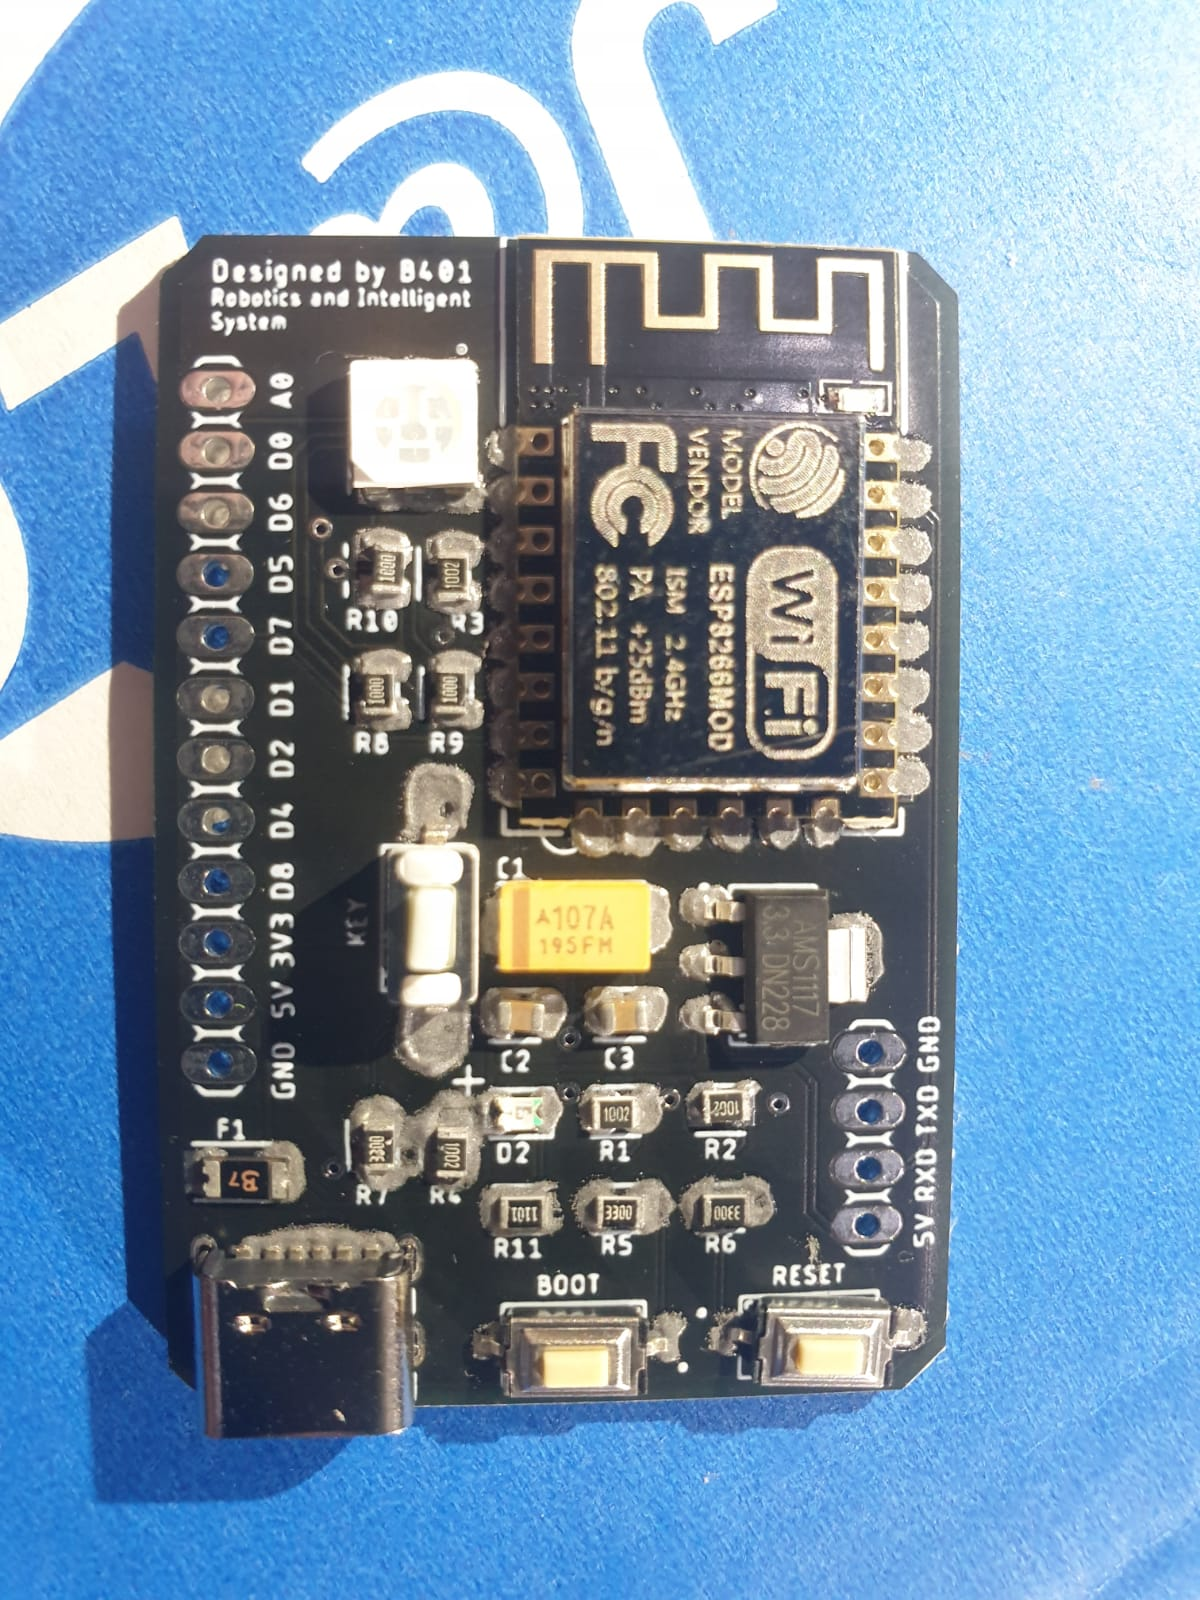
\includegraphics[width=0.4\linewidth]{P4/img/5_tampilan_board_ketika_sudah_dipasang_komponen.jpeg}
        \caption{Tampilan Board Setelah Dipasang Komponen}
        \label{fig:KeadaanBoardSetelahDipasangKomponen}
    \end{figure}
    \item Siapkan solder uap (panaskan solder uap hingga 400$^{\circ}$C).
    \begin{figure}[H]
        \centering
        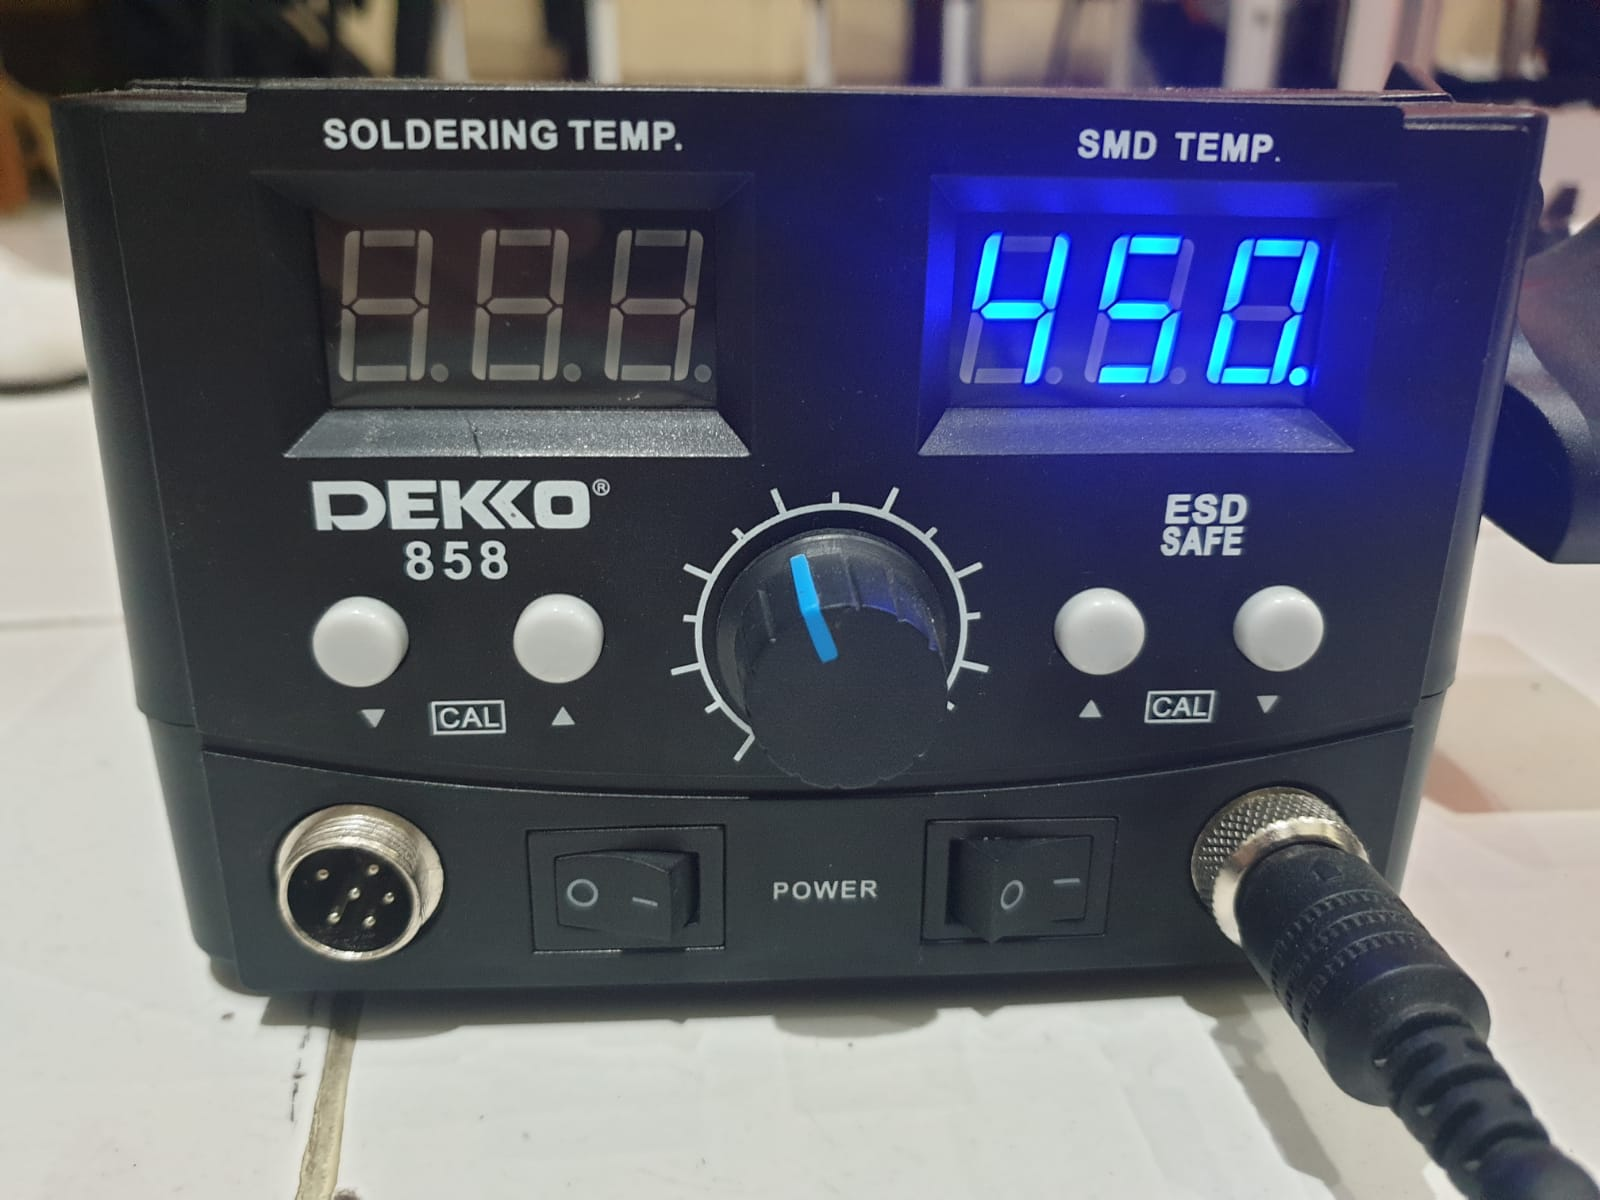
\includegraphics[width=0.4\linewidth]{P4/img/6_pastikan_switch_solder_uap_on_dan_suhu_standart_450.jpeg}
        \caption{Solder Uap On dan Suhu Standart 450$^{\circ}$C}
        \label{fig:SolderUapOn}
    \end{figure}
    \item Solder komponen satu per satu dengan cara dekatkan ujung solder uap ke komponen hingga komponen menempel pada pcb. Pastikan kompone mengering sebelum berpindah ke komponen yang lain.
    \begin{center}
        \colorbox{pink}{\parbox{0.8\linewidth}{\textbf{Tips:} Solder komponen ESP8266 terlebih dahulu.}}
    \end{center}
    \begin{figure}[H]
        \centering
        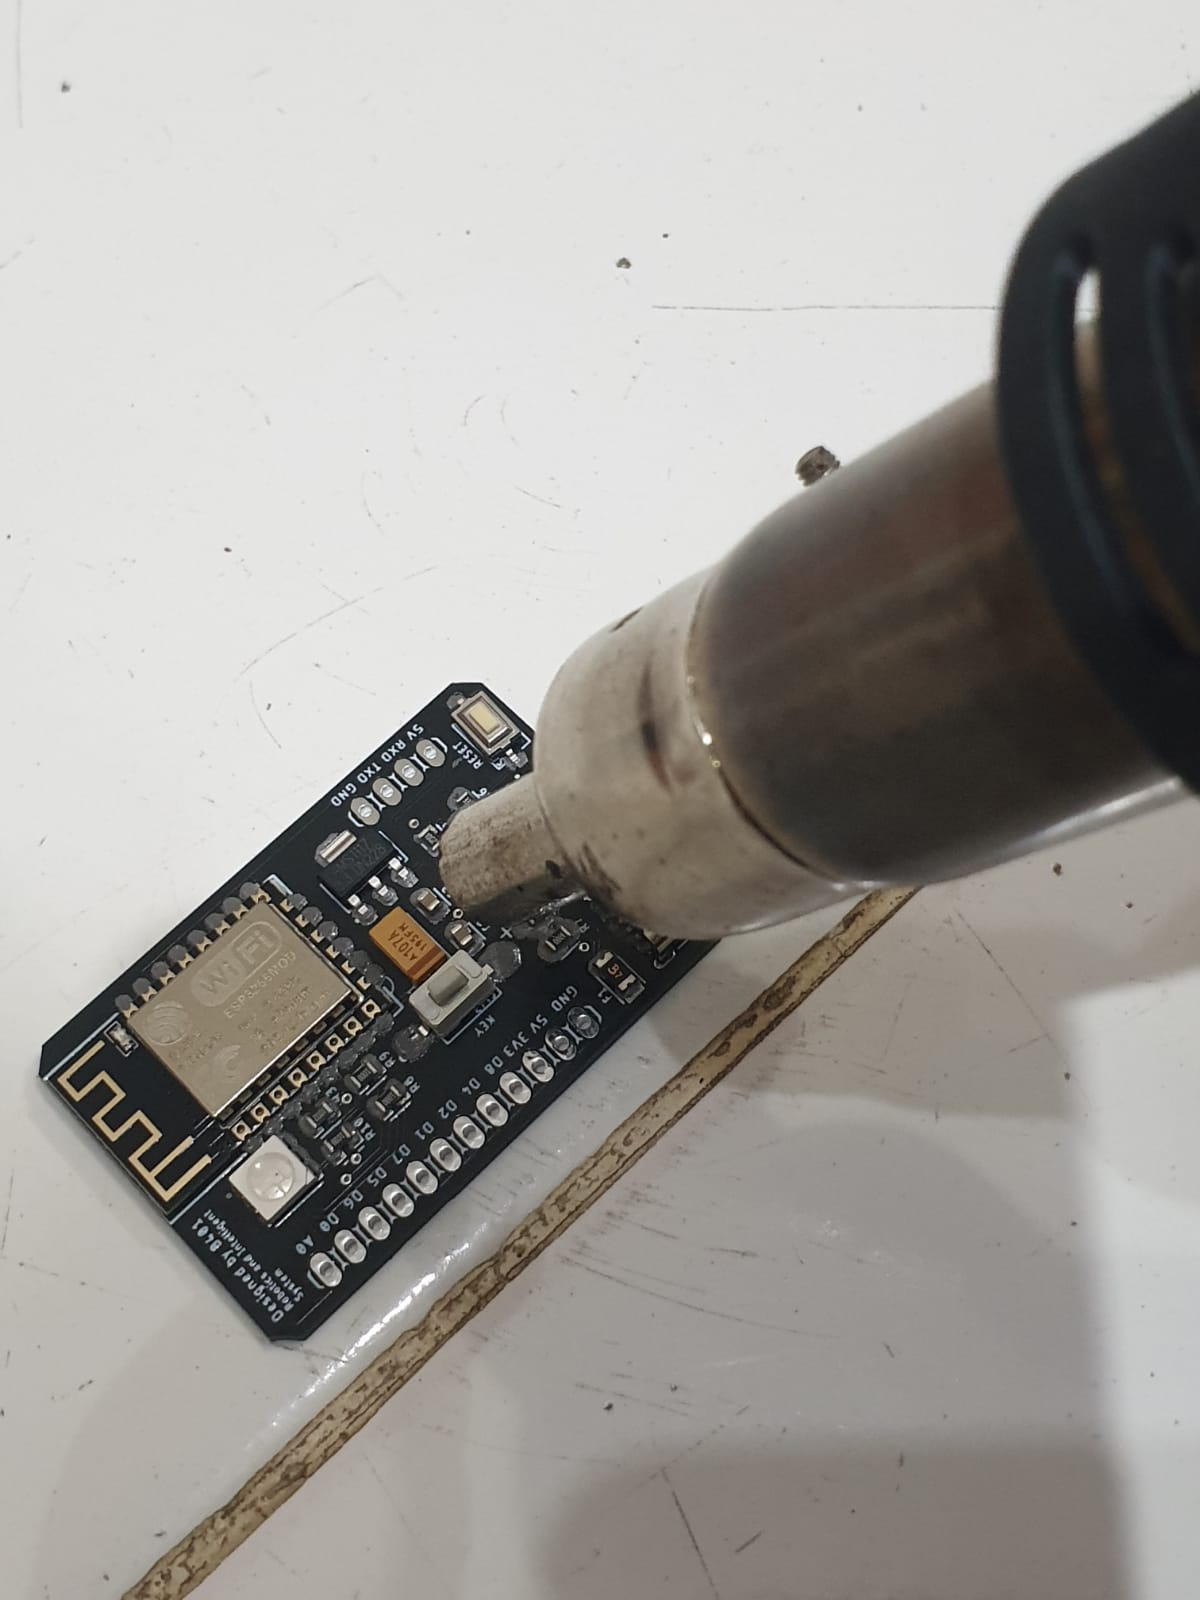
\includegraphics[width=0.4\linewidth]{P4/img/7_posisi_solder_uap_yang_benar.jpeg}
        \caption{Posisi Solder Uap}
        \label{fig:Posisi Solder Uap}
    \end{figure}
    \item Jika sudah selesai pastikan semua komponen sudah terpasang dengan baik.
    \begin{figure}[H]
        \centering
        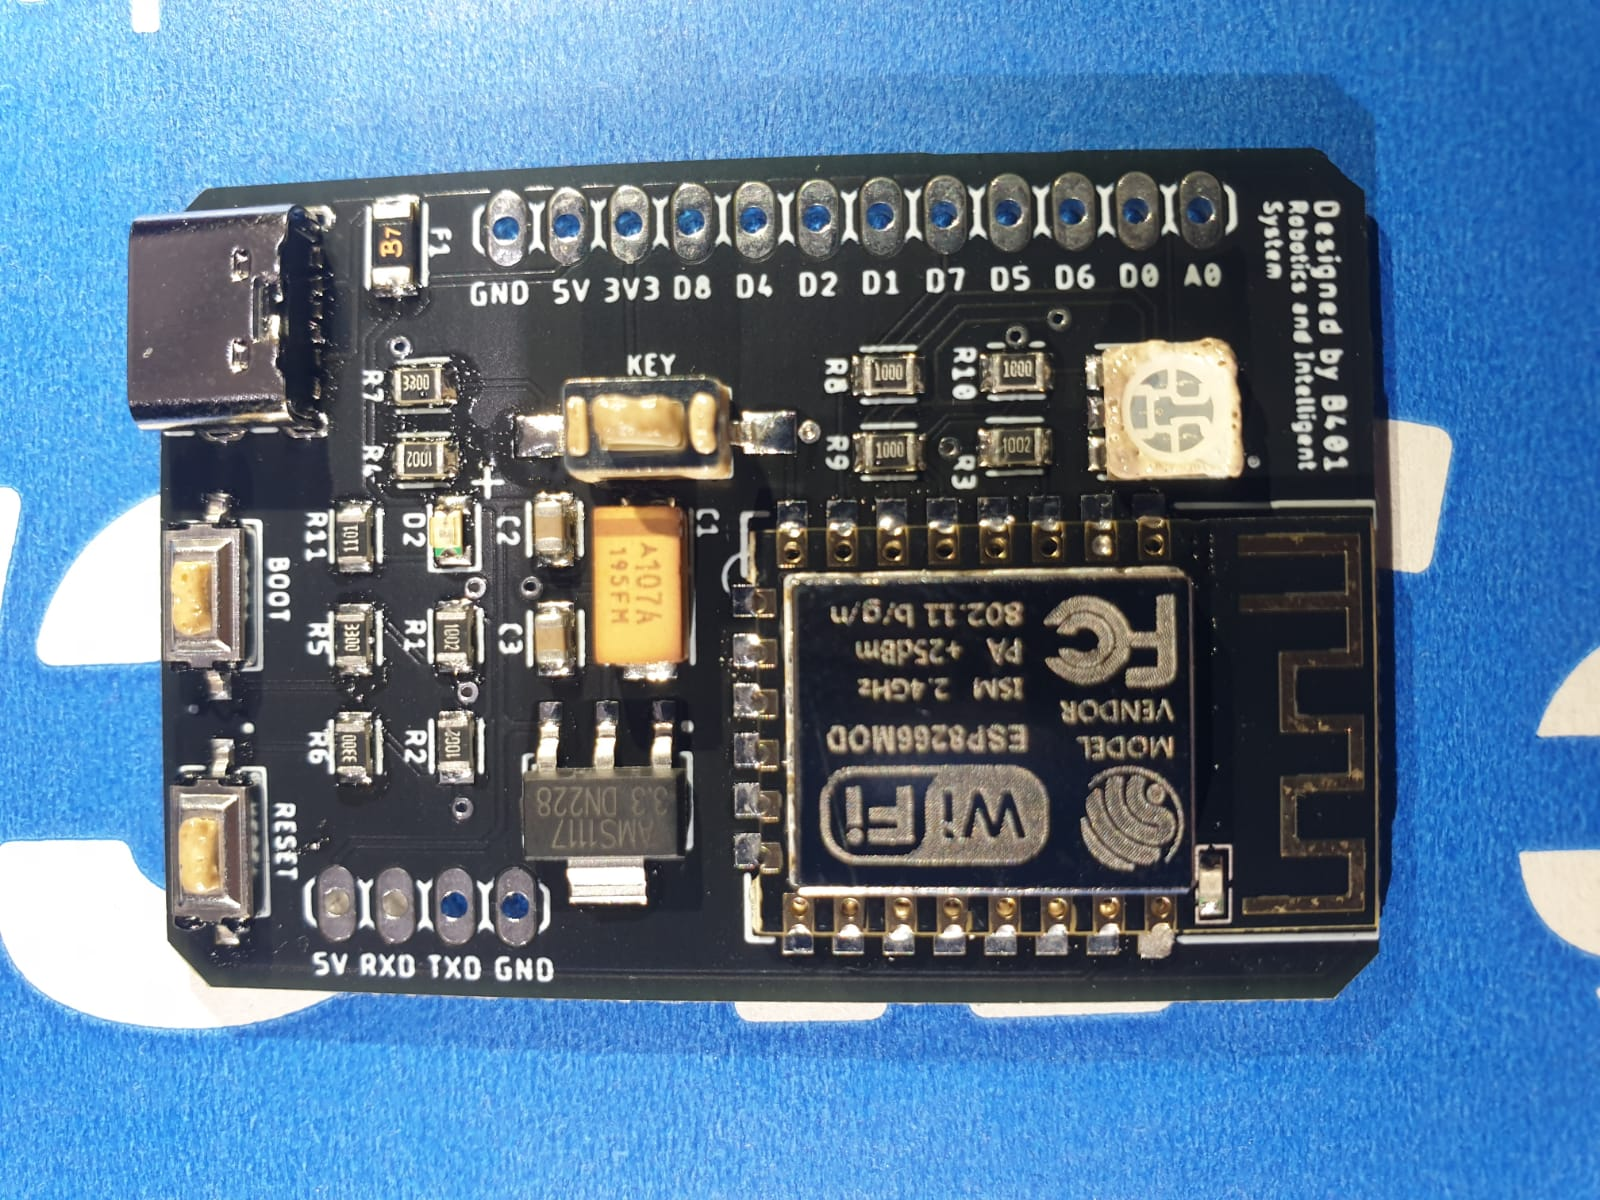
\includegraphics[width=0.4\linewidth]{P4/img/8_keadaan_board_full_komponen.jpeg}
        \caption{Keadaan Board Setelah di Solder}
        \label{fig:KeadaanBoardSetelahSolder}
    \end{figure}
    \item Solder pin header/true hole component dengan timah.
    \begin{figure}[H]
        \centering
        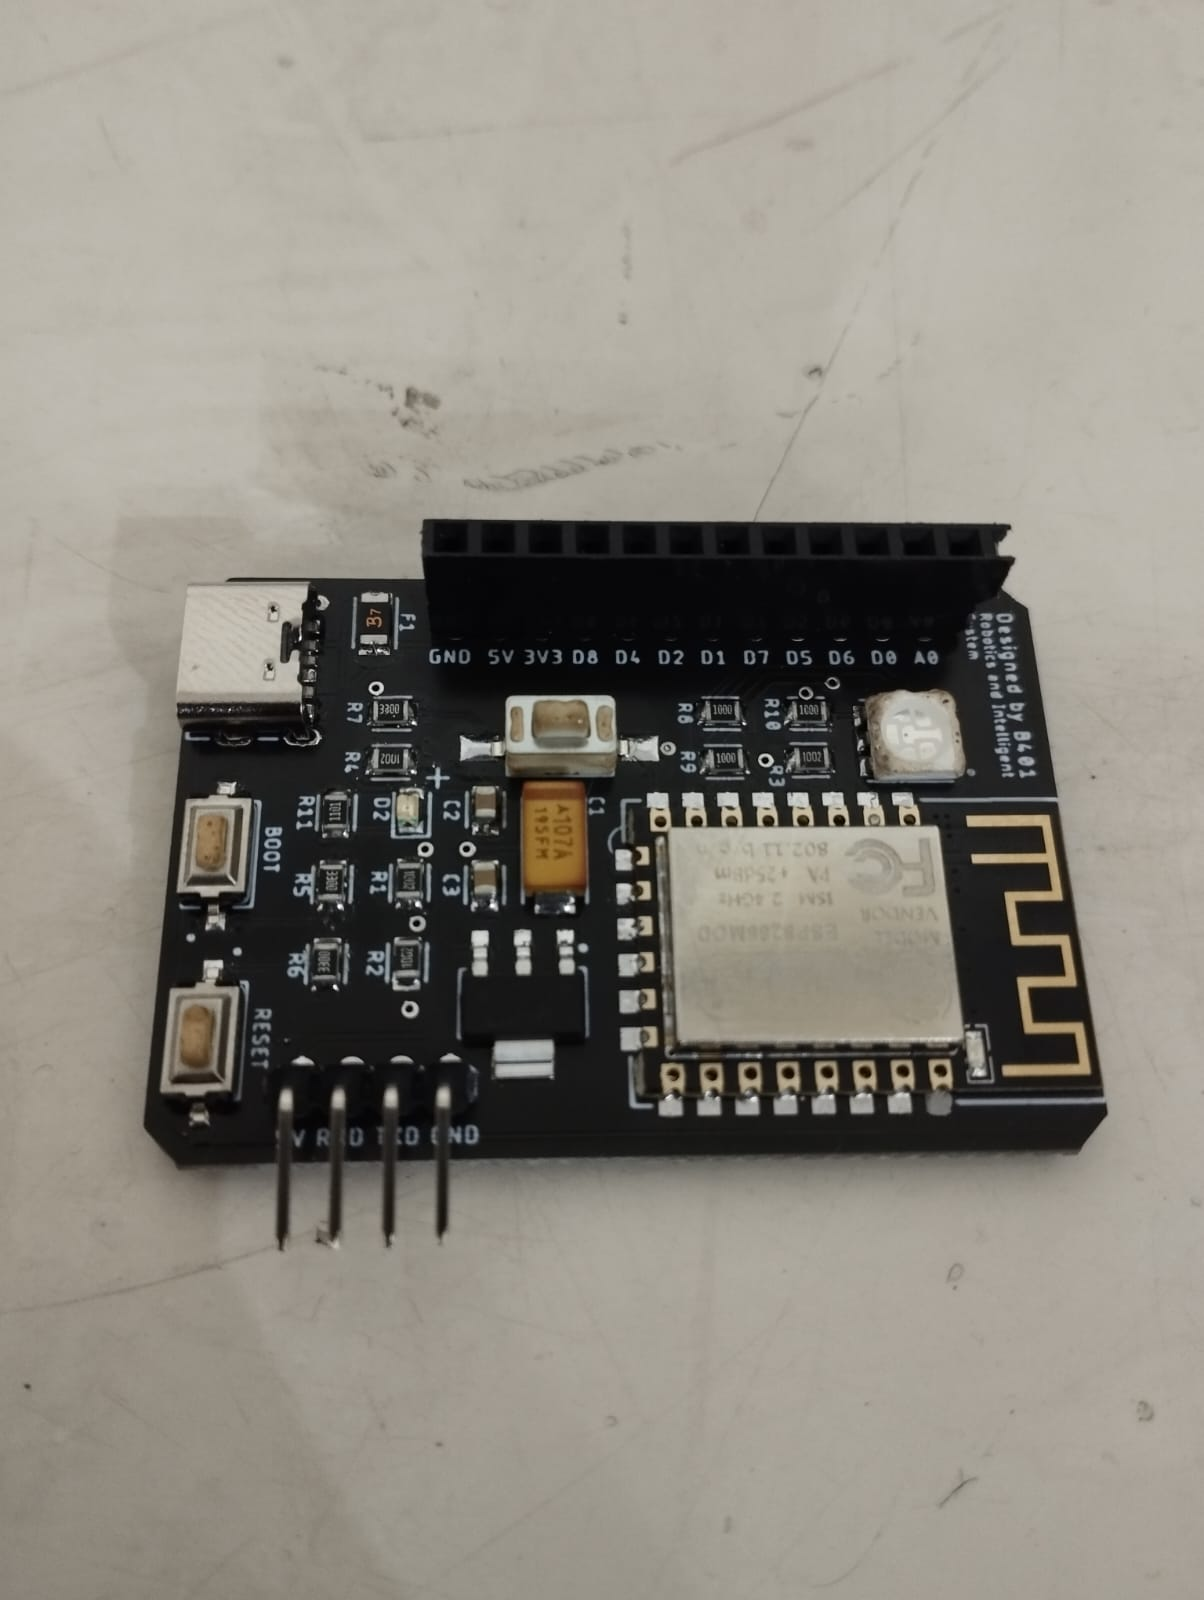
\includegraphics[width=0.4\linewidth]{P4/img/9_keadaan_setelah_disolder_headernya.jpeg}
        \caption{Keadaan Board Setelah Solder Header Pin}
        \label{fig:KeadaanBoardSetelahSolderHeader}
    \end{figure}
\end{enumerate}

\section{Eksperimen 3: Upload Firmware dan Pengujian Fungsional}
\begin{enumerate}
    \item Siapkan modul USB to TTL.
    \item Hubungkan modul ke komputer dan Minimum System ESP8266.
    \begin{figure}[H]
        \centering
        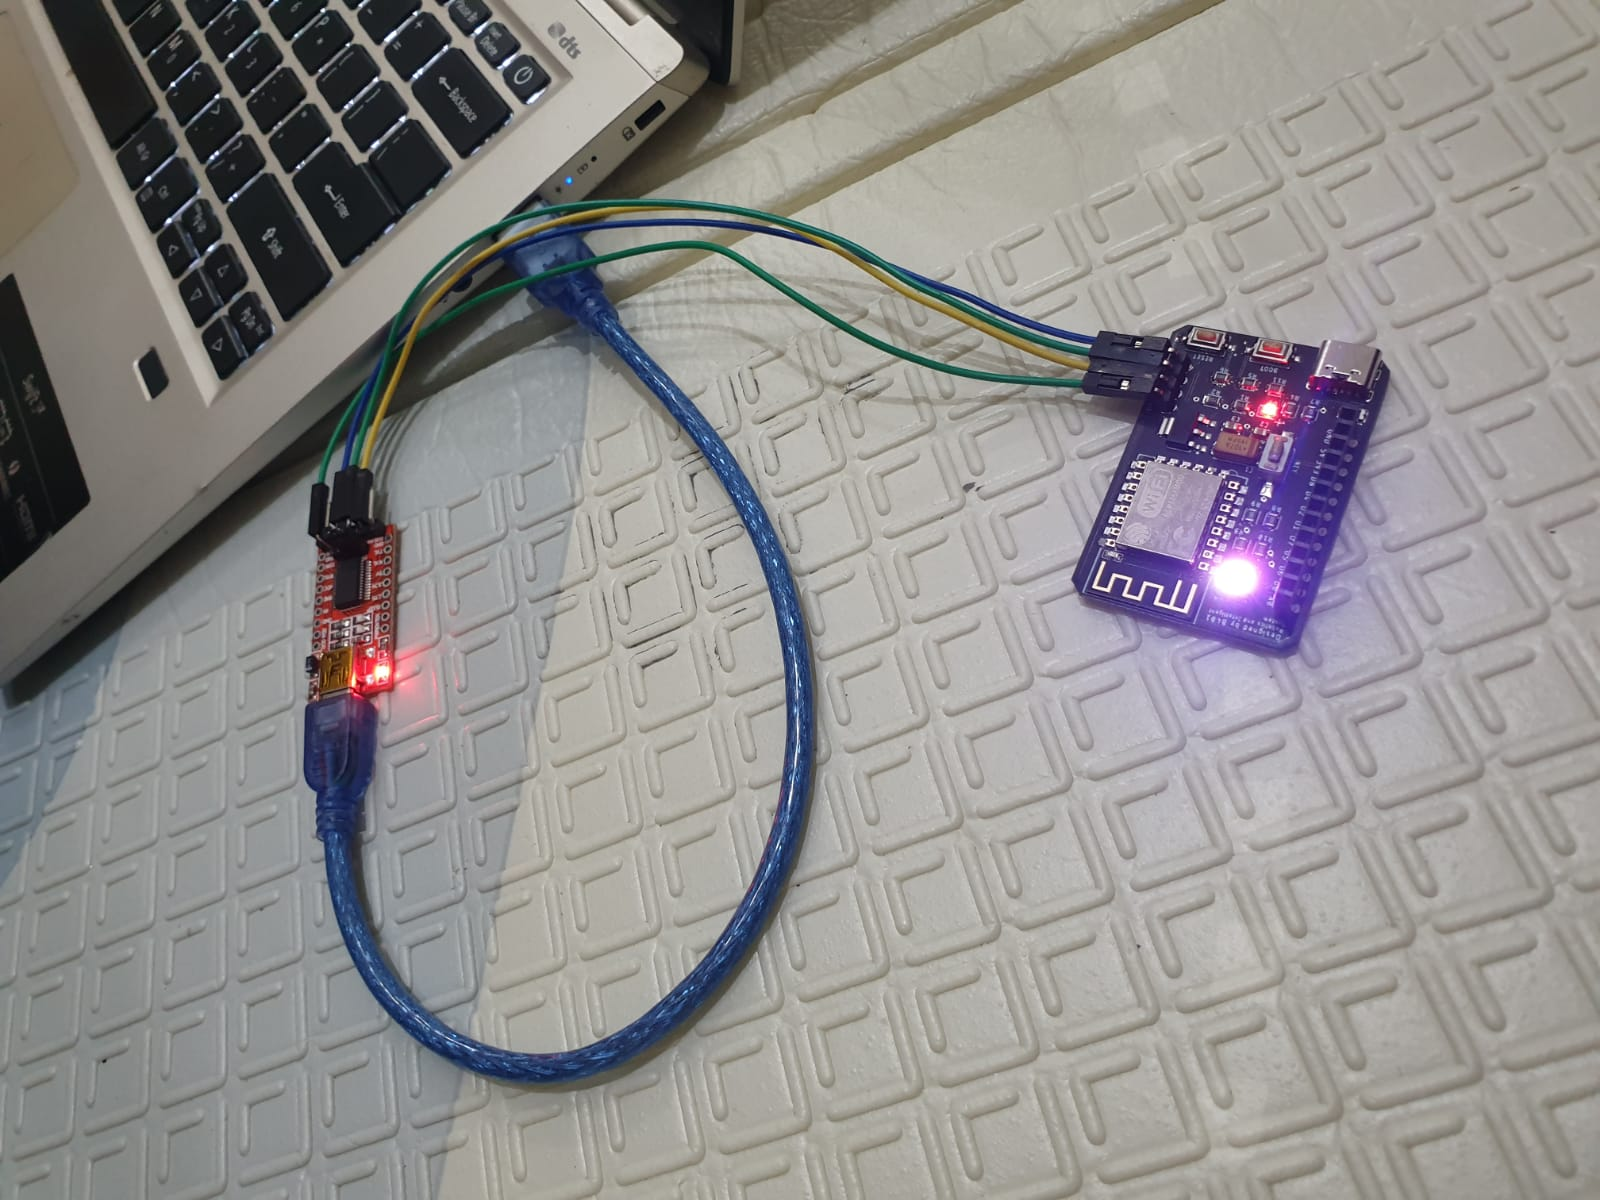
\includegraphics[width=0.4\linewidth]{P4/img/10_hubungkan_dengan_usbttl_dan_laptop.jpeg}
        \caption{USBTTL Dihubungkan ke Laptop}
        \label{fig:USBTTLLaptop}
    \end{figure}
    \item Dowload firmware yang akan digunakan di link berikut: \url{}
    \item Bukalah firmware yang akan dipakai dengan PlatfomIO.
    \item Masuk mode bootloader dengan cara menahan tombol boot dan menekan satu kali tombol reset.
    \item Lepaskan tombol boot.
    \begin{figure}[H]
        \centering
        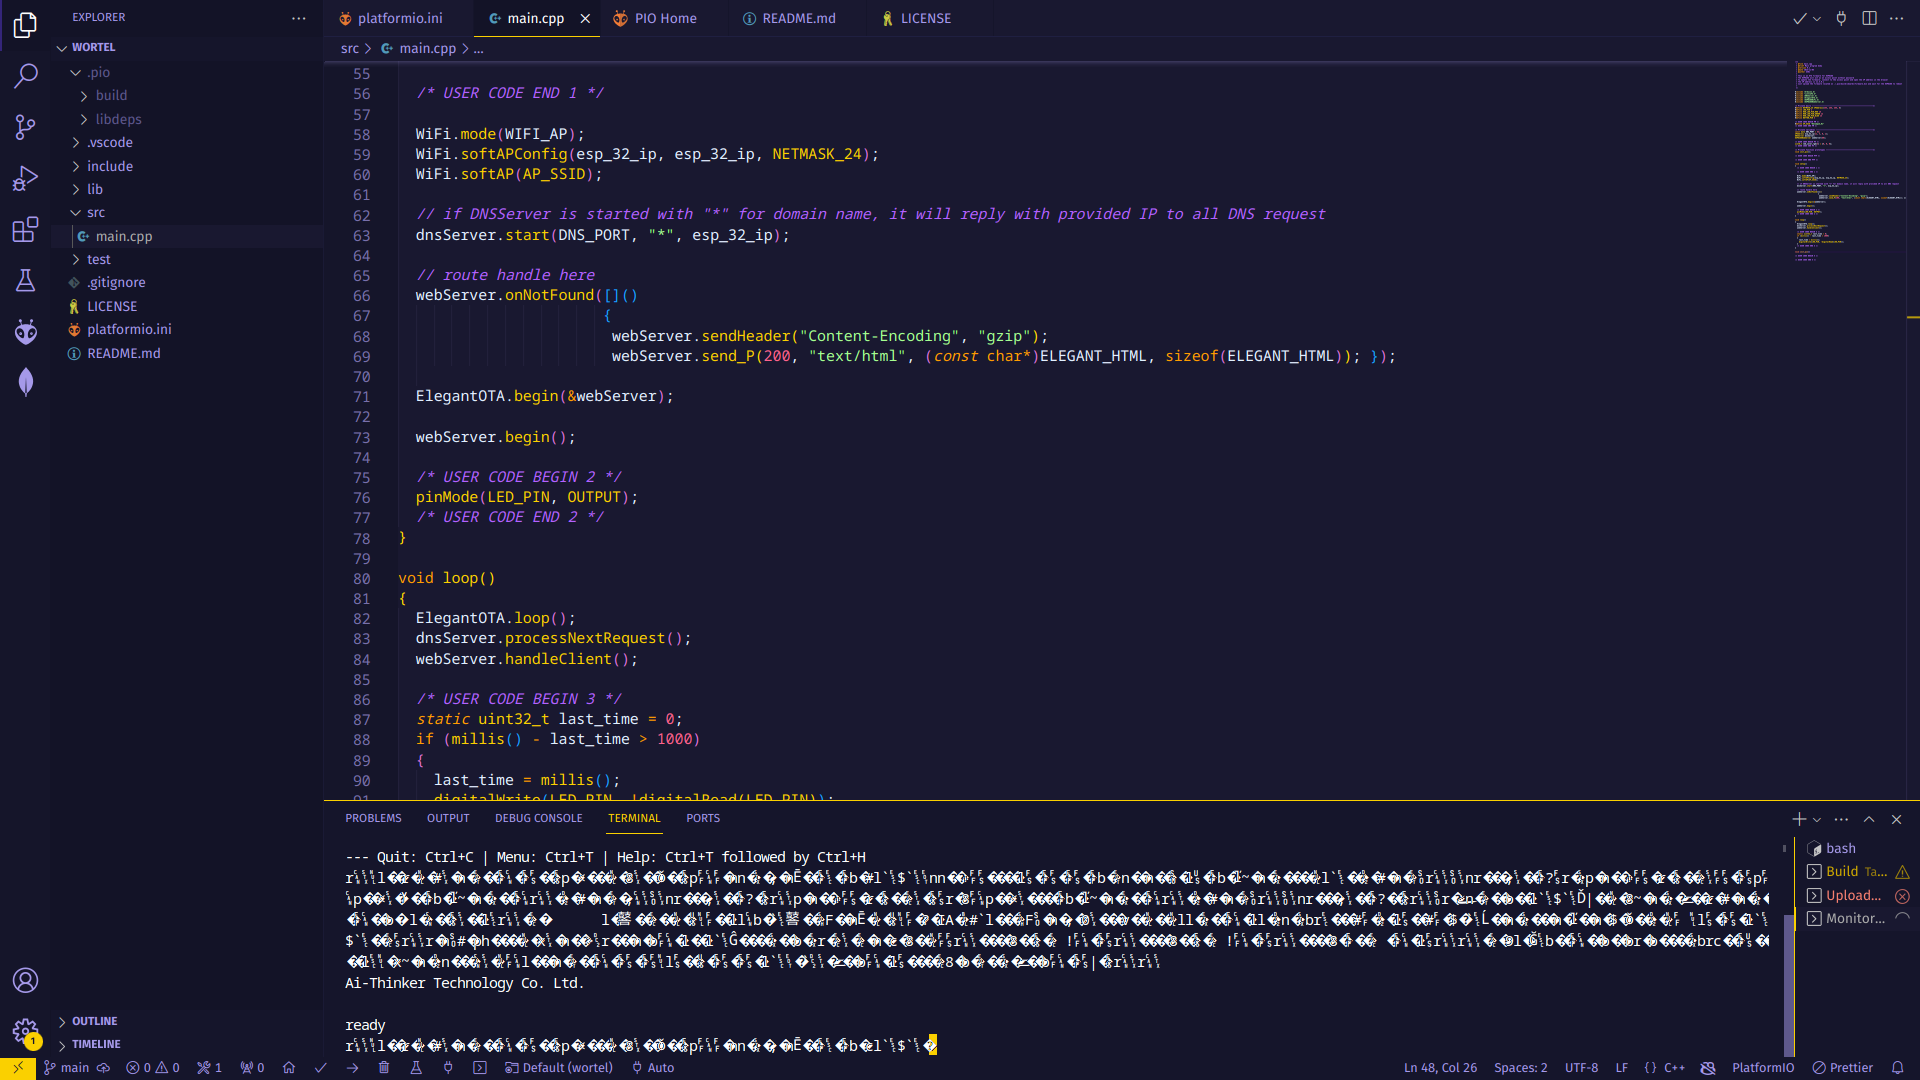
\includegraphics[width=0.4\linewidth]{P4/img/10_tampilan_ketika_esp_masuk_bootloader.png}
        \caption{Tampilan Mode Bootloader}
        \label{fig:TampilanModeBoot}
    \end{figure}
    \item Upload firmware menggunakan PlatformIO.
    \item Tunggu hingga proses upload berhasil.
    \item Jika LED menyala, lanjut ke eksperimen selanjutnya.
    \begin{figure}[H]
        \centering
        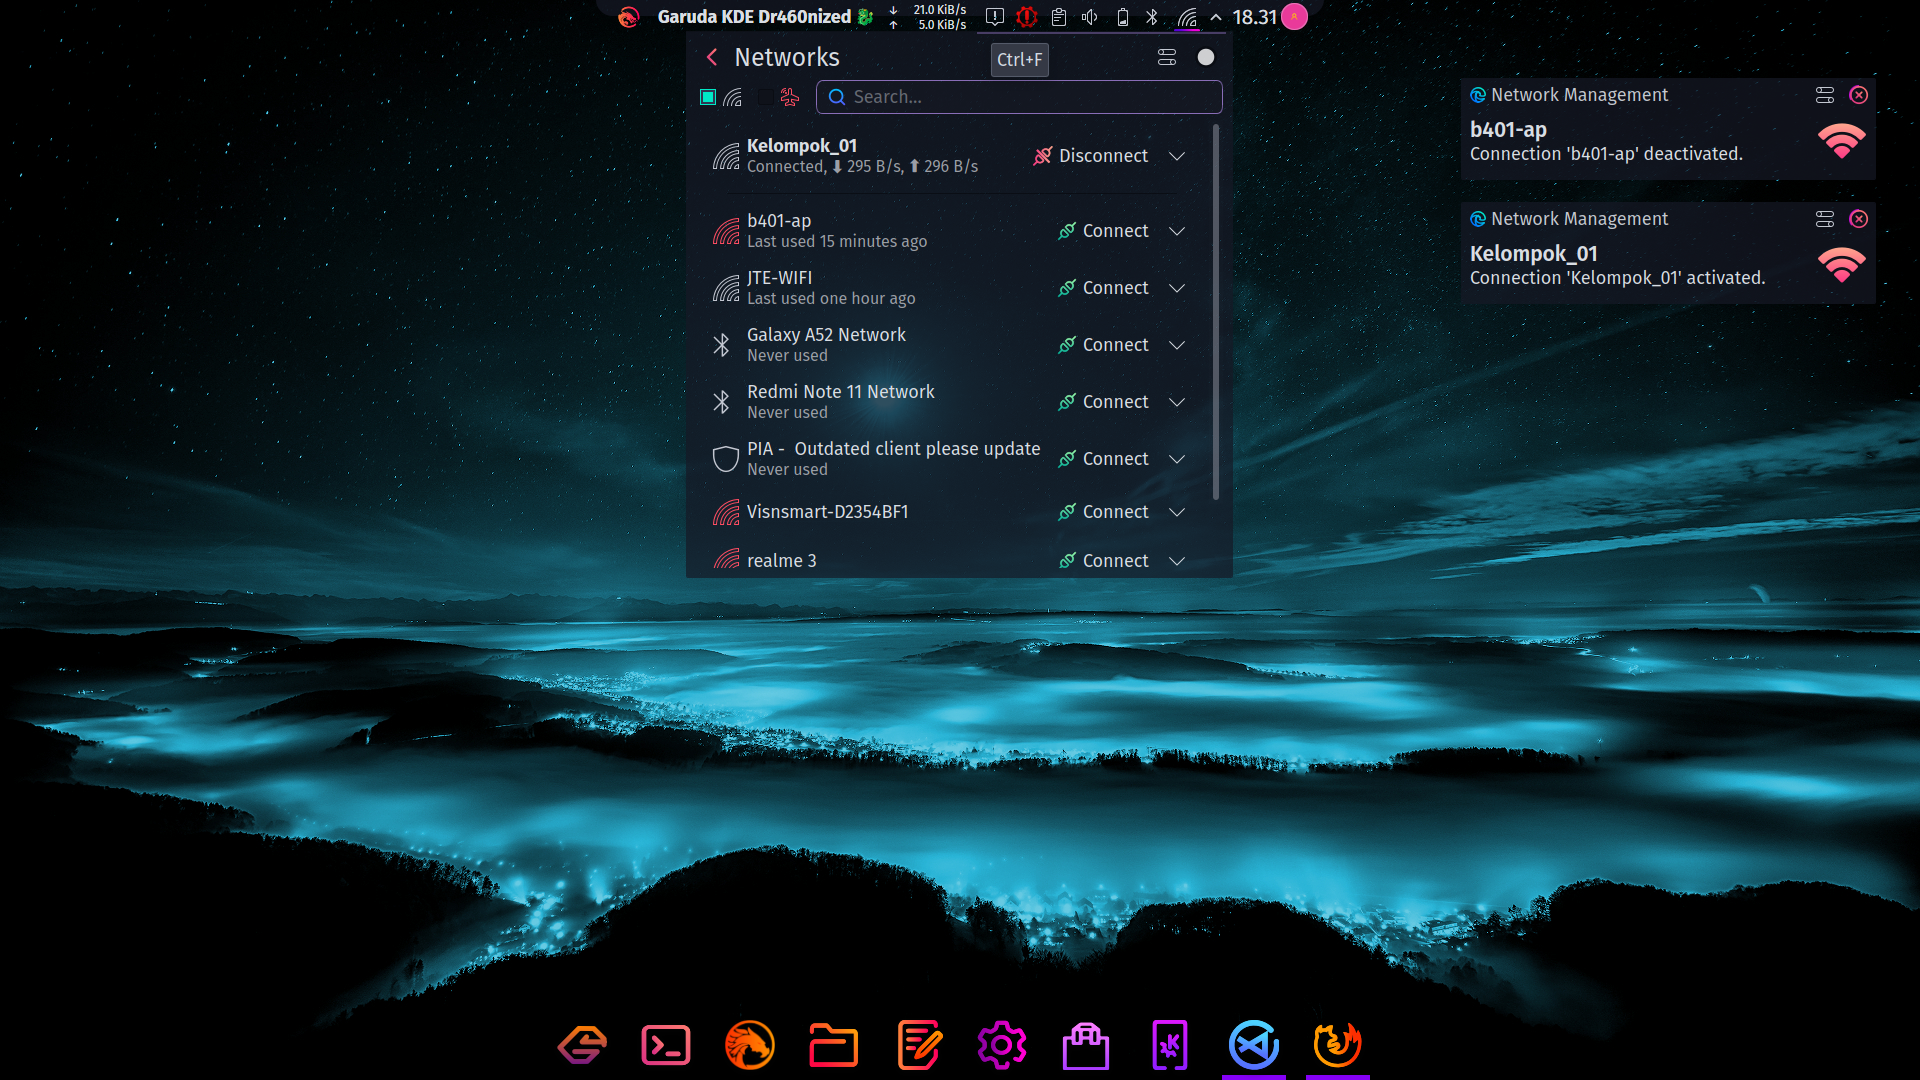
\includegraphics[width=0.4\linewidth]{P4/img/11_tampilan_ssid_ap_ketika_sudah_berhasil_diflash.png}
        \caption{Tampilan SSID AP}
        \label{fig:TampilanSSIDAP}
    \end{figure}
    \begin{figure}[H]
        \centering
        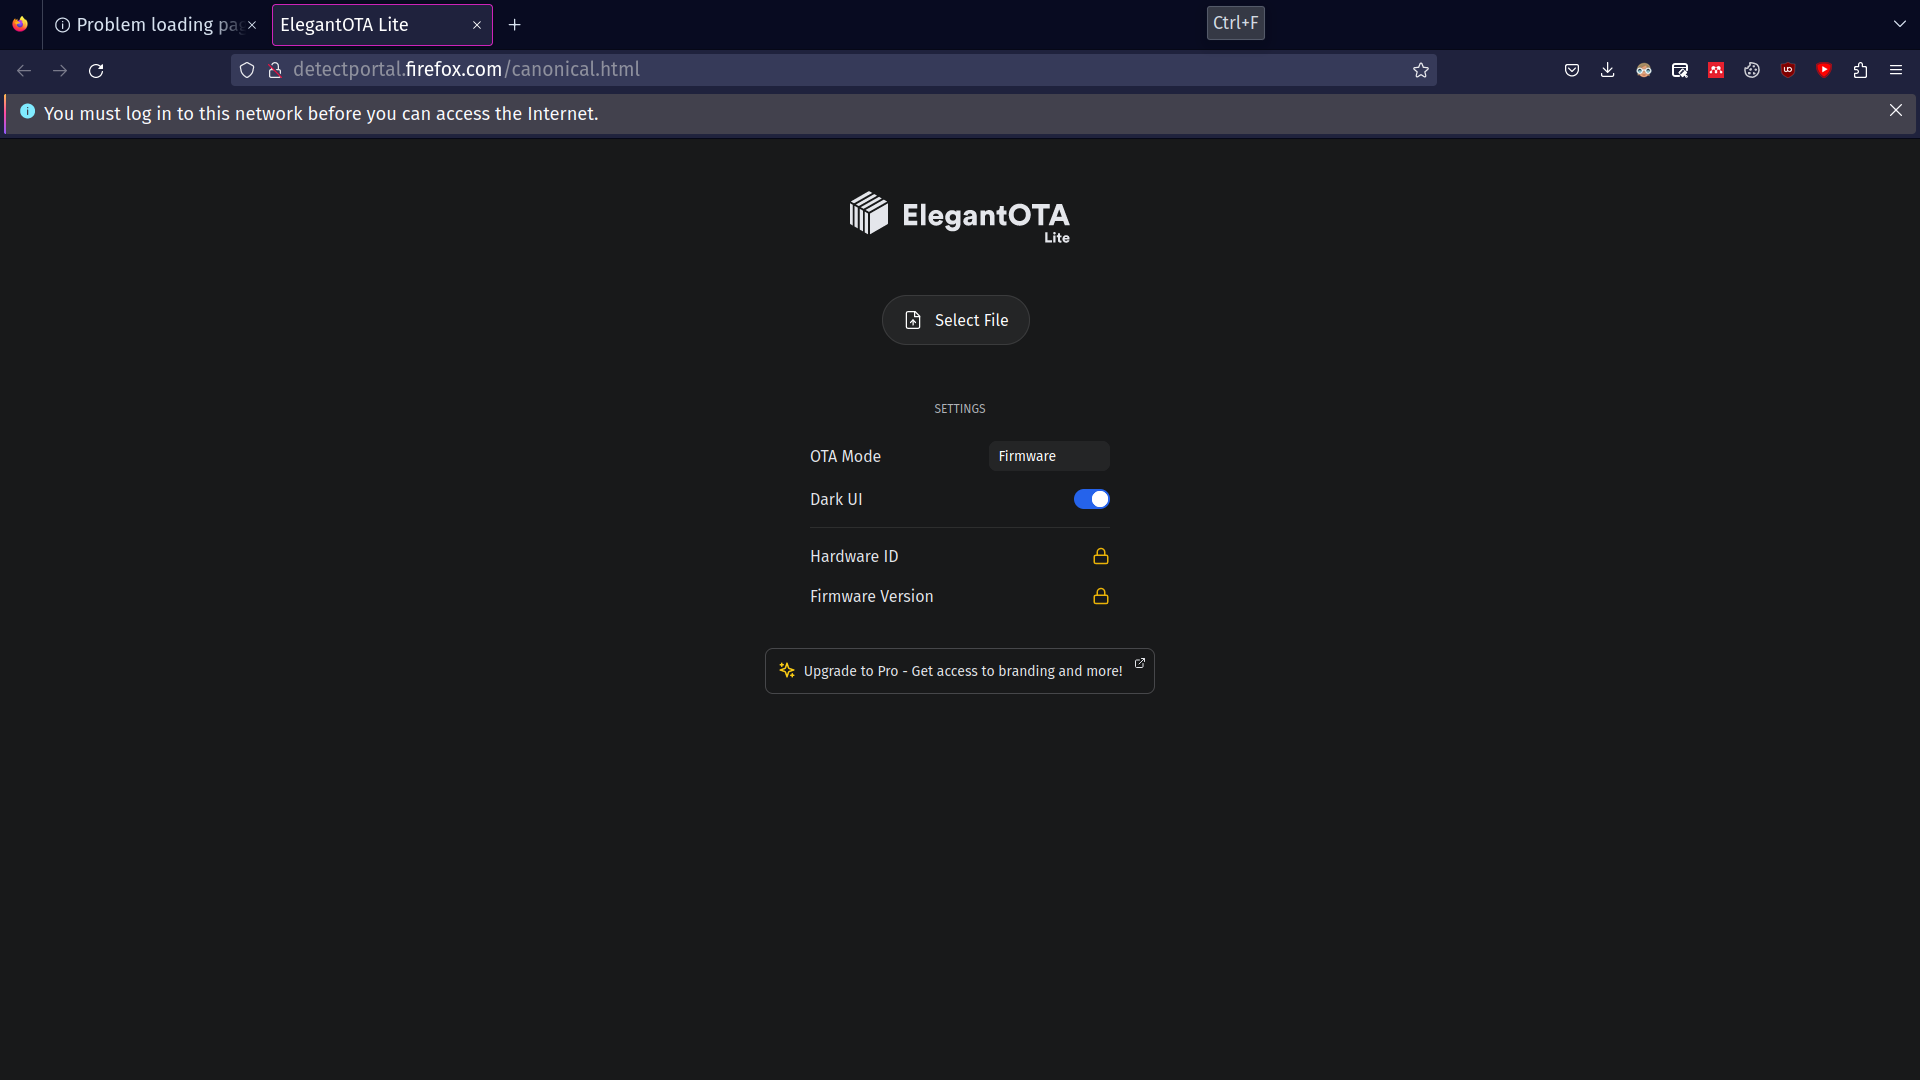
\includegraphics[width=0.4\linewidth]{P4/img/12_tampilan_ota_siap_upload.png}
        \caption{Tampilan OTA}
        \label{fig:Tampilan OTA}
    \end{figure}
    \begin{figure}[H]
        \centering
        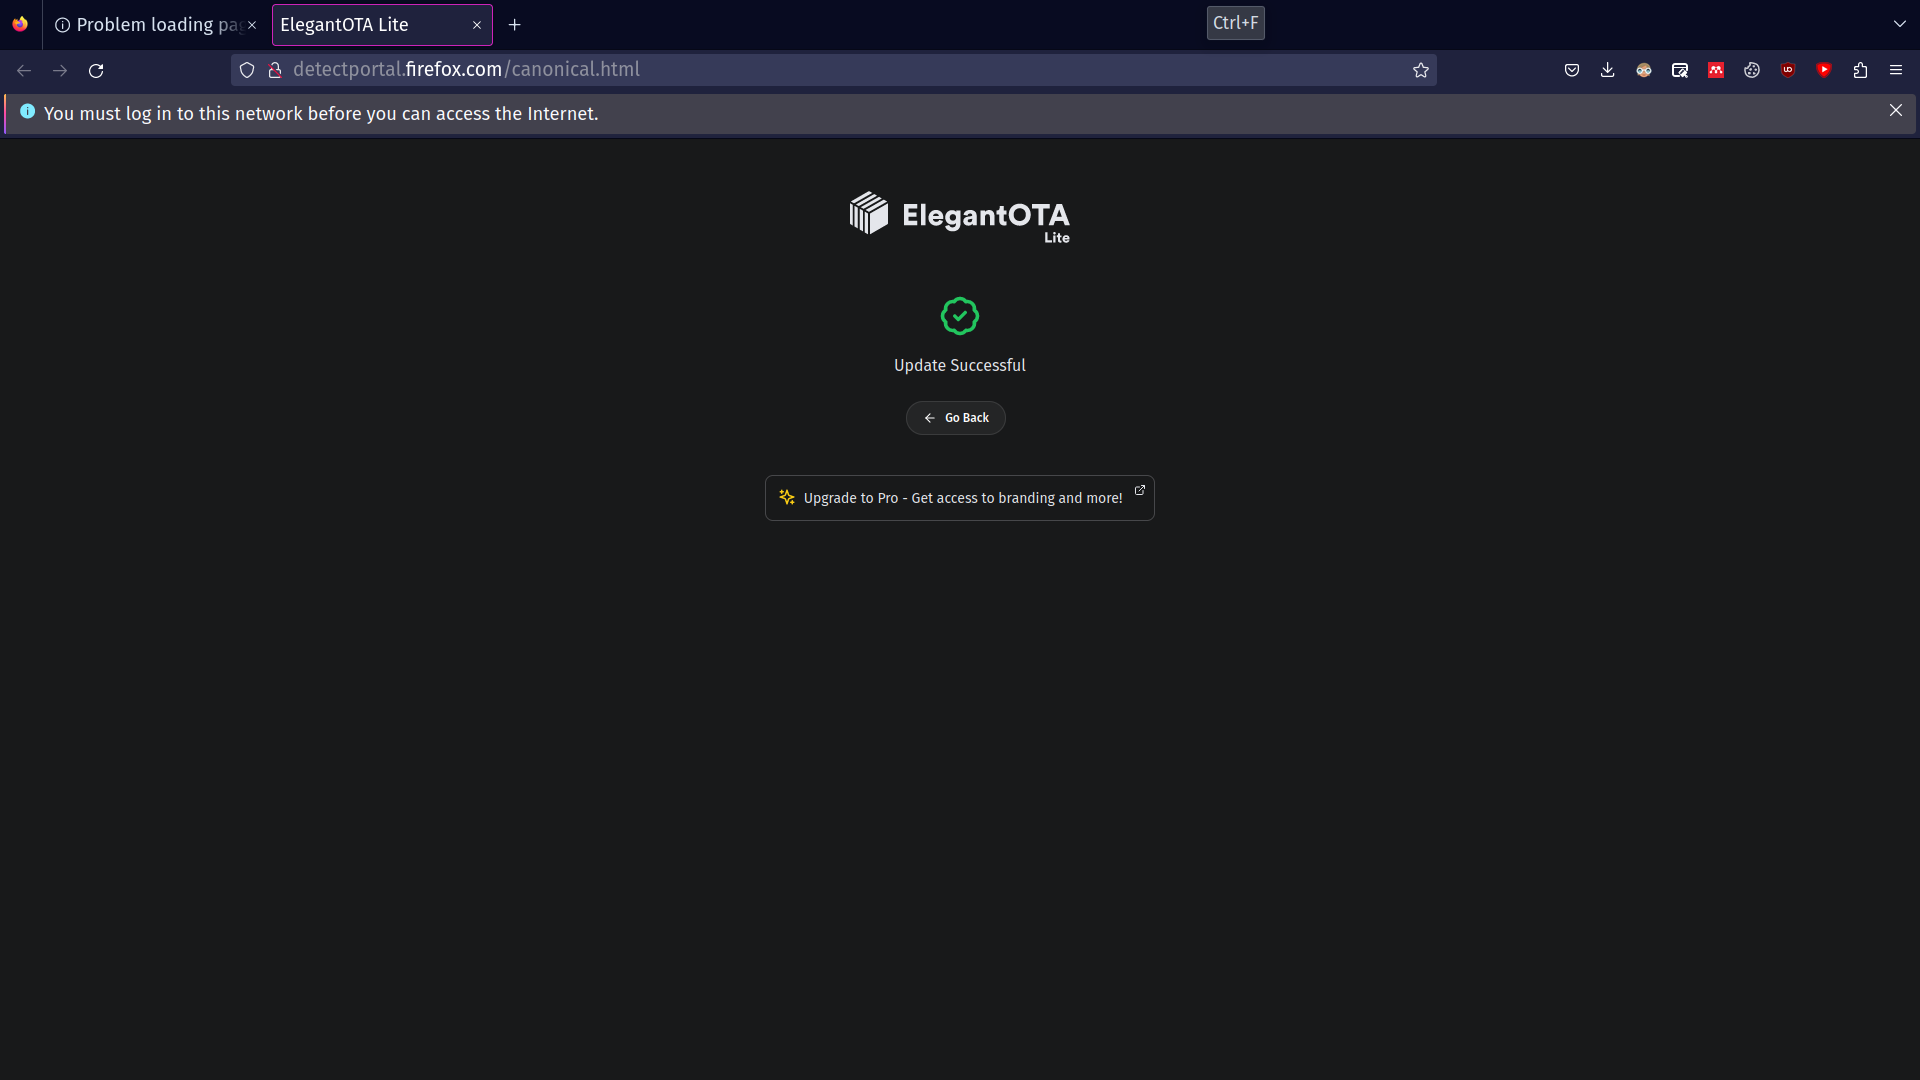
\includegraphics[width=0.4\linewidth]{P4/img/13_tampilan_ota_sukses_upload.png}
        \caption{Tampilan Sukses Upload}
        \label{fig:TampilaSuksesUpload}
    \end{figure}
    \item Jika tidak, ulangi proses upload
    \item Dokumentasikan hasil.
\end{enumerate}

\section{Eksperimen 4: Pengujian Program Kelompok}
\begin{enumerate}
    \item Siapkan program yang akan diuji.
    \item Masukkan program yang sudah dibuat pada template yang sudah disediakan.
    \item Upload program menggunakan PlatformIO.
    \item Tes sesuai dengan klik tombol dan pastikan sesuai dengan hasil yang seharusnya.
    \item Dokumentasikan hasilnya.
\end{enumerate}

